\section{Our Implementation}
We constructed  a simple program, which would take a regular expression and use the methods description in section~\ref{RA_TO_NFA} in to construct a modified NFA structure and use it search for matches using a given pattern.

Our implementation supports a series of regular expression symbols, including $+, ^*, |, ?$ along with concatenation of characters. This allows for construction of simple NFA's from regular expressions, for example the regular expression "(GAT)+" would produce a structure as shown in figure~\ref{fig:gat}

\begin{figure}[h!]
\centering
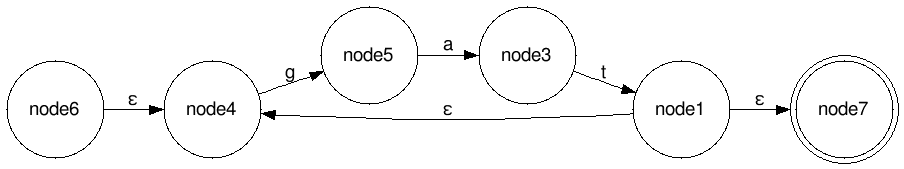
\includegraphics[width=0.5\textwidth]{lib/gat.png}
\caption{Example of how our implementation builds NFA got regular expression (GAT)+}
\label{fig:gat}
\end{figure}

Each node in the figure has a number corresponding to the time it was created in the code, examining figure~\ref{fig:gat} we can see that the NFA part having GAT was constructed first, and then the surrounding nodes responsible for the $+$ were added onto that, much like one would expect from the description in section~\ref{RA_TO_NFA}.

When a NFA is constructed, our implementation will try each possible option when matching, meaning that if there's an epsilon transition it will take it, as well as any other available path. If it cannot match a character directly, but it has the option to handle an insertion or mutation at once, it will take both of them, causing the unmatched state to spawn two new states. This way we can guarantee that we will find every possible match for a given pattern. However it also causes an increased runtime given an increase in mismatches.

One option for optimization could be to make the transition from NFA to Deterministic finite automaton or DFA, which we will not describe in detail here. But as an argument against this, our implementation was made to primarily focus on matching straightforward RNA sequences with insertions, mutations and deletions, which would result in simple linear NFA's, which little to no epsilon transitions. 